\section{Concepts and Terminology}
This section deals with high dimensional spaces (written in mathcal, $\mathcal{Z}$), stochastic variables (written in uppercase $Z$), sets (alsa mathcal), vectors (written as plain variables $z$) and probability distributions (reserving the letter $p$ for this, using indexes to distinguish different distributions).


\section{\acrlong{gans}}
\acrfull{gans} are a family generative models proposed by \textcite{goodfellow2014generative}. The framework for training \acrshort{gans} consists of a data set $\dataset$ with elements in a domain $\dataspace$, a latent space $\latentspace$ and two neural networks, a generator $G(z)$ and a discriminator $D(x)$. The generator maps elements of $\latentspace$ to $\dataspace$, $G: \latentspace \rightarrow \dataspace$. The discriminator is a binary classifier $D: \dataspace \rightarrow [0, 1]$. 

The objective of the discriminator is to classify elements in $\dataspace$ as either members or not members of $\dataset$. Members of $\dataset$ are usually referred to as real samples since they are part of the data set, and non-members are referred to as fake samples. The objective of the generator is to fool the discriminator by mapping elements in $\latentspace$ to the subspace of $\dataspace$ that is classified as real. 

The generator can bee viewed as representing a probability distribution $p_G$ on $\dataspace$. By introducing a latent random variable $Z$ with the probability distribution $p_Z$ on $\latentspace$, the generator probability distribution can be expressed as $p_G(x) = p_Z(G^{-1}(x))$. 

In practice $G^{-1}$ is intractable to compute, whereby explicit probabilities are seldom acquired through \acrshort{gans}. However, this formulation allows sampling from the learned distribution as $G(z), z \sim p_Z$ is straightforward to compute. 

The goal of training \acrshort{gans} is to learn a probability distribution over the data. By viewing the elements of $\dataset$ as outcomes of a random variable $S$ with probability distribution $p_S$ the goal of the generator is to approximate this distribution with $p_G$, and the goal of the discriminator is to discriminate between these distributions. Using this formulation the objective of the \acrshort{gan} training can be formulated as a minimax game 
\begin{equation}
    \min_D \max_G J^{D}(G, D)
\end{equation}
where $J^D(G, D)$ is the discriminator cost function from \parencite{goodfellow2016nips},
\begin{equation}
    J^D(G, D) = -\frac{1}{2}\mathbb{E}_{x \sim p_S, z \sim p_Z}\left[\log(D(x)) - \log(1 - D(G(z))) \right].
    \label{eq:GANcost}
\end{equation}
%\begin{equation}
%    \mathcal{L}(x_1, x_2) = -\log(D(x)) + \log(D(x_2)), \quad \begin{cases} x \in X \\ z \in \latentspace \end{cases}.
%\end{equation}
Since both the generator and discriminator are differentiable functions, (\ref{eq:GANcost}) can be optimized using standard gradient based optimization schemes such as RMSprop \parencite{tieleman2012lecture} or Adam \parencite{kingma2014adam}. Typically the networks are updated in an alternating fashion where the parameters of one of the networks are frozen while updating the other network. The expectectations in (\ref{eq:GANcost}) are typically estimated using minibatches as 
\begin{equation}
    \mathbb{E}_{x\sim p(x)}[f(x)] \approx \frac{1}{m}\sum_{i=1}^mf(x_i)
\end{equation}
where $x_i$ is sampled from $p(x)$. This process is described in an algorithmic fashion in Algorithm \ref{alg:GANbase}.

\begin{algorithm}
    \caption{Training scheme for \acrlong{gans}}
  \label{alg:GANbase}
  \begin{algorithmic}[1]
    \STATE operation 0 \label{op0}
    \STATE operation 1 \label{op1}
  \end{algorithmic}
\end{algorithm}

\begin{figure}
    \caption{An illustration of GANs}
    \label{fig:GAN}
    \centering
    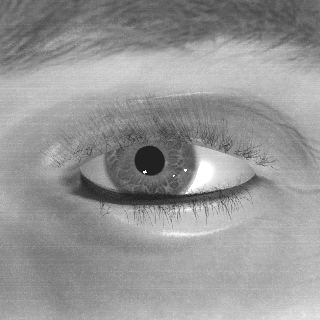
\includegraphics[width=0.3\textwidth]{banana.png}
\end{figure}

\subsection{Theoretical analysis of \acrshort{gans}}
In the original paper (\textcite{goodfellow2014generative}) a couple of theoretical properties of \acrshort{gans} are formulated and proved. These proofs assume that both the generator and discriminator have infinite capacity.

Firstly it is proven that given a fixed generator $G$ the optimal discriminator is 
\begin{equation}
    D(x) = \frac{p_S(X=x)}{p_S(X=x) + p_G(X=x)}.
\end{equation}
A straightforward implication of this is that when $G$ is optimal, the optimal $D$ always output $0.5$ for all real and fake data points. In other words
\begin{equation}
    p_G \eqdist p_S \implies D(x) = 0.5 \; \forall x \sim p_G, p_S
\end{equation}
if $D$ and $G$ are optimal. Secondly, it is also proved in the original paper that given an optimal discriminator there exists aglobal maximum of the discriminator cost function and it is reached if and only if $p_G \eqdist p_S$. Finally convergence of the training algorithm (Algorithm \ref{alg:GANbase}) is proven.

\subsection{Practical issues}
The theoretical results indicate that \acrshort{gans} are a sensible method for implicitly learning probability distributions. However when implementing GANs in practice some issues emerge from using models of finite capacity. 

Training stability issues...

Gradient descent not guaranteed convergence: "Previous approaches to GAN training have thus applied gradient descent on each player’s cost simultaneously, despite the lack of guarantee that this procedure will converge." \textcite{salimans2016improved}.

Mode collapse...

Another issue encountered when implementing \acrshort{gans} in practice emerges from the limitations of representing a continous distribution with a finite data set. Even though the theoretical results guarantee $p_G$ converges to $p_S$, $p_S$ is not uniquely determined. In fact, $p_S$ is represented by sampling from a uniform discrete distribution over the data set $\dataset$. Therefore the optimal generator would theoretically collapse to this discrete distribution. This results in a generator incapable of generalizing to new data points. On the other hand, should this behaviour be encoutered in practice with limited capacity, the model would still be usable as a compression of the data for applications that only require sampling from the data set. An example for this is using the generator as a proxy for the data set during training or evaluation of another neural network.

\subsection{Variantions}
Since the introduction of \acrshort{gans}, several variations and extensions have been proposed to overcome some of the original issues. A few of these are outlined in this section.

\subsubsection{Non Saturating \acrshort{gan}} 
An issue with training \acrshort{gans} on the original discriminator cost function (\ref{eq:GANcost}) is that the adversarial term $\log(1-D(G(Z)))$ saturates if the discriminator is too confident. This can prevent the generator from learning in the beginning when the generator output are quite dissimilar to the original data. In the original article it is suggested to train the generator to minimize $-\log(D(G(Z))$ instead. This cost is sometimes reffered to as the non saturating const function.

The non saturating cost function preserves the fixed point dynamics of the original \acrshort{gan} formulation while at the same time permitting the generator to learn when the discriminator is confident. Due to this property, non saturating \acrshort{gans} are the implementation used for the experiments in the original article.

\subsubsection{Conditional \acrshort{gan}}
A limitation of the \acrshort{gan} framework is that it does not allow external information such as image annotations to be modeled. A straightforward extension of the original framework is to let the generator model the conditional distribution $p_S(X|Y)$, where $Y$ represents the additional information. This was proposed in the original article, and was later formally introduced and tested on MNIST\footnote{\textcite{lecun2010mnist}} by \textcite{mirza2014conditional}. The conditional distributions are modeled by introducing the additional information as input to both the discriminator and the classifier.


\subsubsection{Auxiliary Classifier GAN}
The Auxiliary Classifier GAN, proposed by \textcite{odena2016conditional}, is another approach of modelling conditional distributions with \acrshort{gans}. As in the normal conditional \acrshort{gan}, the generator recieves an outcome from both the latent variable $Z$ and the conditional variable $Y$ and generates a sample from this information. In this case the conditional variable is assumed to be a class label, but the approach is easily extendible. In contrast to the generator, the discriminator only recieves the generated sample without any class label. Instead, the discriminator simultaneously attempts to discriminate between real and fake images, as well as producing label class probabilities.

In this framework, the generator is trained to simultaneously produce data points that yields confident correct class predictions at the same time as they are indistinguishable from the correct data points. This approach have been shown to generate images with state of the art Inception score at the time \parencite{odena2016conditional}.

A problem with this constellation is that the generator is biased towards learning to generate images that can easily be classified. This means that the optimal discriminator doesn't necessarily provide $p_G \eqdist p_S$. It has been shown that the distribution bias introduced by this model causes the generator to completely avoid generating ones with serifs when trained on MNIST despite the high frequency of serifed ones in the data set \textcite{shuac2017acganisbad}.

\subsubsection{BiGAN}
Can utilize the latent space.
\subsubsection{WGAN}
A popular alternative to traditional GAN training is the Wasserstein \acrshort{gan}. It was proposed n 2017 by \textcite{arjovsky2017wasserstein}.

\subsubsection{BEGAN}
\subsubsection{DRAGAN}
\subsubsection{Progressive GAN}

\subsection{Difficulties when training GANs}
Arjovsky showed that NSGAN generator has a weird objective given an optimal discriminator \textcite{arjovsky2017towards}.
They do not need to decrease a divergence at each step \textcite{fedus2017many}.

\subsection{Evaluating the performance of GANs}
Are all GANs created equal? \textcite{lucic2017gans}

Problem with inception score on AC-GAN \textcite{shuac2017acganisbad}



\section{\acrlong{vaes}}
Another popular family of generative models besides \acrshort{gans} are \acrfull{vaes}. \acrlong{vaes} were first introduced by \textcite{kingma2013auto} as a scalable approach for stochastic variational inference. \acrshort{vaes} are trained using the \acrfull{aevb} algorithm proposed in the same article. 

These models consists of an i.i.d. data set $\dataset$ and a continous latent variable $Z$ in a latent space $\latentspace$. The data set is viewed as a set of outcomes of a random variable $S$ as previously. The prior $p(Z)$ and likelihood $p(S|Z)$ are assumed to come from parametric families of distributions and the posterior $p(Z|S)$ is assumed to be intractable and is modeled by some parametric distribution. The parameters of the prior and likelihood distribution are commonly denoted as the generative model parameters $\theta$. The probabilities in the context of these model are commonly denoted as $p_\theta(X)$, $p_\theta(X|Z)$ and $p_\theta(Z|X)$ to explicitly expose the model parameters. Since the posterior $p_\theta(Z|X)$ is assumed intractable it is estimated with a variational approximation, commonly denoted $q_\phi(Z|X)$. From the deep learning perspective, $q_\phi(Z|X)$ is commonly refered to as the \textit{encoder}, and $p_\theta(X|Z)$ is commonly referred to as the \textit{decoder}.

The \acrshort{aevb} algorithm is applied to learn the generative model parameters and infer the optimal variational parameters. It is a type of approximate variational inference and consists of gradient based optimization of an estimatior of the variational lower bound of the marginal likelihood of the data under the current model. In the original article the authors propose the two estimators based on Monte Carlo estimates of expectations:
\begin{equation}
    \begin{aligned}
        \mathcal{L}^A = \frac{1}{L}\sum_{l=1}^L \log p_\theta (X=x^{(i)},Z=z^{(i, l)}) - \log q_\phi (Z=z^{(i, l)} | X=x^{(i)}) ), \\
        \mathcal{L}^B = - D_{KL}(q_\phi (Z | X=x^{(i)}) || p_\theta(Z=z)) + \frac{1}{L}\sum_{l=1}^L \log p_\theta (X=x^{(i)},Z=z^{(i, l)}).
    \end{aligned}
\end{equation}

\begin{algorithm}
    \caption{Training scheme for \acrlong{vaes}}
  \label{alg:VAEbase}
  \begin{algorithmic}[1]
    \STATE operation 0 \label{op0}
    \STATE operation 1 \label{op1}
  \end{algorithmic}
\end{algorithm}

\begin{figure}
    \caption{Variational autoencoder}
    \label{fig:VAE}
    \centering
    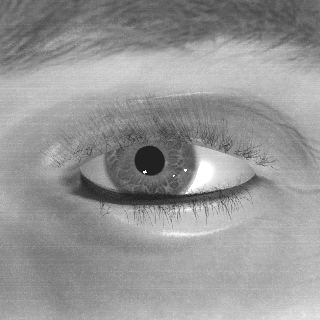
\includegraphics[width=0.3\textwidth]{banana.png}
\end{figure}

\acrshort{vaes} can be trained by maximizing either of these estimates using common gradient based methods as described in Algorithm \ref{alg:VAEbase}. An issue at the moment is that the lower bound estimates require sampling from the latent variable, which is a non-differentiable operation. \textcite{kingma2013auto} resolved this issue by introducing a reparametrization trick to enable gradients to flow through the sampling process. This is applied in Algorithm \ref{alg:VAEbase}, but will not be explained in detail in this report for brevity. The illustrations in \parencite{doersch2016tutorial} are an excellent source of intuition why this works.

\subsection{Similarities with \acrshort{gans}}
Both \acrshort{vaes} and \acrshort{gans} implicitly model the data distribution $p_S(x)$ by introducing a latent stochastic variable Z

Combination of VAE and GAN: VAEGAN. \textcite{LarsenSW15autoencodingbeyond}

\section{Semi-supervised learning}
Formulate problem, go through some apporaches.

Improved GAN, go through vanilla version and combination with self training \cite{wuliu2017selftrainsemisup}

\section{Image-to-Image Models}

\section{Common architectures}

\section{Normalization techniques}

\section{Related work}
Hmm, värt att nämna? 






